\chapter{Implementace software}
Software je rozdělen na čtyři moduly. Každý modul v sobě uzavírá specifickou funkcionalitu. Hlavním modulem je modul core, kde je veškerá logika programu. Ostatní moduly už jsou jen pro uživatelské rozhraní, které je případně možné implementovat i jinak např. je možné udělat webové rozhraní.
\section{Modul Core}
Modul core je jádro celého programu, uzavírá v sobě funkcionalitu pro načítání algoritmů, práci s obrazem, generování výstupních souboru a práci s více vlákny. Na obrázku \ref{fig:core_whole} je vidět základní schéma modulu. Modul je rozdělen do několika balíčku, z nichž stěžejní jsou algorithm, video, task a output. Ostatní balíčky obsahuje pomocné třídy, jako jsou různé utility třídy, DTO, vyjímky, ...

V modulu core je ještě několik tříd, které nejsou zařazené do žádného balíčku. Třída EnvLoader má na starost správné načtení konkrétních knihoven pro danou platformu, jelikož knihovna OpenCV využívá nativní knihovny zkompilované pro každou platformu zvlášť a v Jave jsou tyto knihovny volány přes \gls{glos:JNA}, tak je nutné načíst nativní knihovny do systému. Momentálně je v programu podporována platforma Windows x86 a x64.

Další třídou je BMAThreadFactory, která implementuje rozhraní ThreadFactory. Třída slouží, jako factory pro executor servise. Vlákna, která se zde vytvoří, jsou řazena pod jednu skupinu a ta může mít svůj volitelný název. Všechna vlákna jsou pak vytvořena s prioritou normal a neběží v režimu "démon". Veškerá práce s vlákny v programu pak probíhá pomocí ExecutorService, kde je využito BMAThreadFactory pro tvorbu nových vláken.

\begin{figure}[h]
	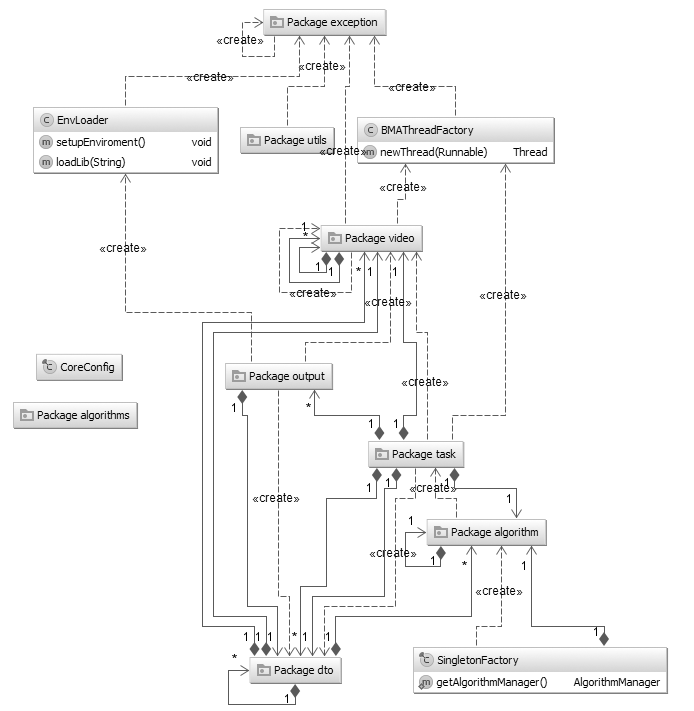
\includegraphics[scale=1]{core_whole}
	\centering
	\caption{Modul core \label{fig:core_whole}}
\end{figure} 
\FloatBarrier
\subsection{Balíček Algorithm}
V balíčku algorithm, jehož schéma je vidět na obrázku \ref{fig:core_algorithm}, je funkcionalita pro načítání počáteční konfigurace algoritmu a práci s načteními algoritmy. Veškerou funkcionalitu balíčku v sobě uzavírá třída AlgorithmManager, přes kterou se volá AlgorithmService a také v sobě drží aktuálně načtené algoritmy. V programu se vytváří pouze jedna singleton instance manageru a ta se pak získává přes SingletonFactory.

\begin{figure}[h]
	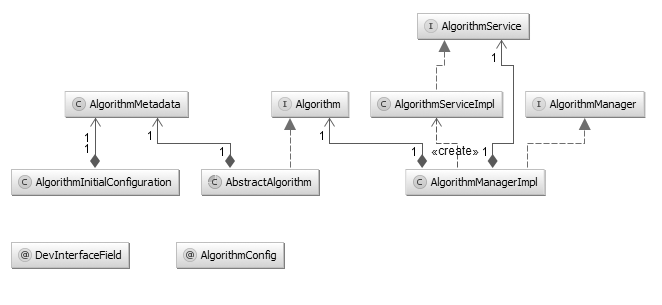
\includegraphics[scale=0.8]{core_algorithm}
	\centering
	\caption{Balíček algorithm \label{fig:core_algorithm}}
\end{figure} 
\FloatBarrier
Pro vytvoření nového algoritmu je nutné, aby nová třída implementovala rozhraní Algorithm nebo dědila již od základní implementace AbstractAlgorithm. Dále může volitelně obsahovat třídu, která slouží jako konfigurace algoritmu. Tato třída musí mít anotaci AlgorithmConfig. V konfiguraci je pak možné anotovat jednotlivé atributy anotací DevInterfaceField, ty pak budou na základě konfigurace v anotaci vidět ve vývojovém rozhraní. Konkrétní nastavení algoritmu je uloženo v externím XML souboru, který je mapován na třídu AlgorithmInitialConfiguration. Díky tomu je možné mít více algoritmů s různou konfigurací. Ukázka nového algoritmu je zobrazena na obrázku \ref{fig:core_new}. Načtení algoritmu pak probíhá následovně:
\begin{enumerate}
	\item Procházení všech XML souborů.
	\item Soubor je rozmaršálován na třídu AlgorithmInitialConfiguration pomocí JAXB.
	\item Pomocí reflexe je nalezena a vytvořena nová instance třídy, která je uvedena v className, viz. obrázek \ref{fig:core_new}.
	\item Nastavení metadat algoritmu.
	\item Vytvoření nové konfigurace algoritmu a nastavení atributů na základě hodnot v XML. Vše je pak dosazeno do instance třídy pomocí reflexe.
	\item Vložení inicializovaného algoritmu do mapy k ostatním algoritmům.
\end{enumerate}

\begin{figure}[h]
	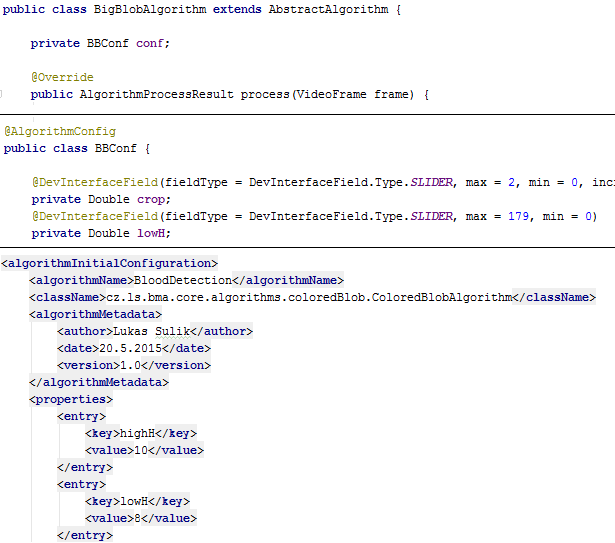
\includegraphics[scale=0.9]{core_new}
	\centering
	\caption{Ukázka nového algoritmu \label{fig:core_new}}
\end{figure} 
\FloatBarrier

\subsection{Balíček Video}
V balíčku video jsou pouze dvě třídy: Buffer a VideoFrame. VideoFrame je třída, která slouží k uchovávání informace o jednom obrazovém rámci. Má v sobě matici, která reprezentuje obrázek, číslo rámce a zámek. Zámek je zde proto, že se s rámcem pracuje ve více vláknech a je nutné poznat, zdali už byl rámec zpracován všemi algoritmy. Zámek je vyjádřen třídou AtomicInteger a je to číselná hodnota, která se nastavuje vždy při vytváření rámce (popsáno níže), a jedná se o vyjádření počtu algoritmů, které s ním budou pracovat. Po zpracování algoritmem se hodnota zámku sníží o jedna. VideoFrame také obsahuje pomocnou funkcionalitu pro vývojové rozhraní, tato funkcionalita je aktivní pouze pokud je vývojové rozhraní aktivní. Vývojová funkcionalita umožňuje dočasně ukládat matice z průběhu zpracování algoritmu do mapy, ale tato možnost funguje pouze pro jedno vlákno.

Třída Buffer slouží, jak již název napovídá, jako zásobník pro VideoFrame. Samotný zásobník je řešen pomocí rozhraní ConcurrentNavigableMap a konkrétní implementace ConcurrentSkipListMap. S touto třídou je možno pracovat na více vláknech bez rizika deadlocku. Pořadí hodnot v mapě je tříděno přirozeně pomocí klíče a datová struktura skip list umožňuje rychlé vyhledávání v mapě dle klíče. Velikost bufferu se dá řídit definovanou konstantou, po naplnění bufferu nelze přidávat další elementy. To zajišťuje metoda addFrame, která slouží pro vytvoření a vložení nového framu, pokud je již buffer naplněn tak nelze nový frame přidat. Čištění bufferu probíhá automaticky. Při vytvoření objektu je spuštěna čistící sekvence, která odmazává všechny framy s nulovou hodnotou zámku. Sekvence běží do té doby, než je buffer uzavřen a je prázdný. Uzavření bufferu je stav, kdy už do něj nelze přidat další hodnoty, stav je reprezentován atributem typu boolean.

\subsection{Balíček Task}
Další částí programu je balíček Task, jehož schéma je vidět na obrázku \ref{fig:core_task}. Třídy v něm obsažené slouží k vykonávání asynchronních úkolů a implementují buď Runnable nebo Callable, v případě, že je potřeba čekat na výsledek. V třídách grabber je načítání souborů z disku. Jak název napovídá tak buď videa, anebo celé složky (kde se načítají obrázky). K načtení je v obou případech použita knihovna OpenCV, která načte jednotlivé soubory a udělá z nich matice ve formátu BGR (pouze přeházené kanály o proti RGB, jinak je formát stejný). Načtená matice je pak vložena do třídy buffer, kde bude čekat na další zpracování.

Pro zpracování videa se využívá třída AlgorithmTask, která je potomkem AbstractBufferTask. V této třídě dochází ke zpracování dat algoritmem, metody pro sběr dat jsou definovány v abstraktním předkovi. Po vytažení dat se spustí metoda algoritmu, která zjistí, jestli se v konkrétním snímku nachází nějaká anomálie. V případě pozitivního výsledku se snímek uloží do přepravky, která se pak použije při generování výstupu. Jakmile je operace dokončena, z video snímku se odstraní zámek pro konkrétní algoritmus a pošle se signál pro aktualizaci průběhu.

\begin{figure}[h]
	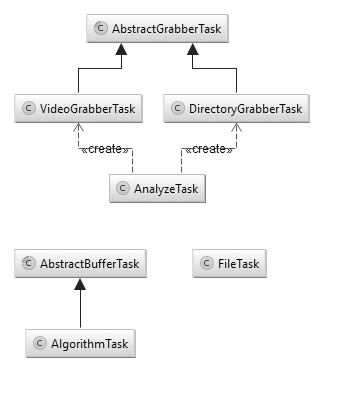
\includegraphics[scale=0.9]{core_task}
	\centering
	\caption{Balíček Task \label{fig:core_task}}
\end{figure} 
\FloatBarrier

Třída AnalyzeTask spojuje funkcionalitu všech předchozích tasku. Pro každý soubor se vytvoří buffer a spustí se GrabberTask na novém vlákně. Jakmile je GrabberTask zapnut, tak se vyžádají od AlgorithmManagera všechny aktivní algoritmy a jejich tasky, kde se použije tentýž buffer. Ty se poté také spustí asynchronně. Z důvodu optimalizace bylo přidáno omezení na zpracování maximálně dvou souborů/složek zároveň. I to ale občas může způsobovat problémy, tak do budoucího rozvoje práce by bylo dobré zlepšit optimalizace, např. použít knihovnu MapDB. Po dokončení všech operací se pošle signál k aktualizaci průběhu a vygeneruje se přepravka s výsledky analýzy.

\subsection{Balíček Output}
Poslední hlavní částí modulu Core je balíček output. Ten má v sobě obsaženou logiku pro generování výstupních souborů. V současné době je podporován formát XLSX a PDF. Generováni obou formátů je řešené podobně, každý formát však obsahuje specifické nástroje pro tvorbu. Schéma pro tvorbu XLSX je vidět na obrázku \ref{fig:core_output}. Aplikace komunikuje s generátory pomocí rozhraní FileOutput. V rámci generování XLSX(i PDF) se vnitřní logika rozpadne na několik menších generátorů, které implementují rozhraní XLSXGenerator (případně PDFGenerator). Tyto generátory se pak spustí v hlavní třídě XLSXOutput v předem daném pořadí a vznikne tak výsledný soubor.

\begin{figure}[h]
	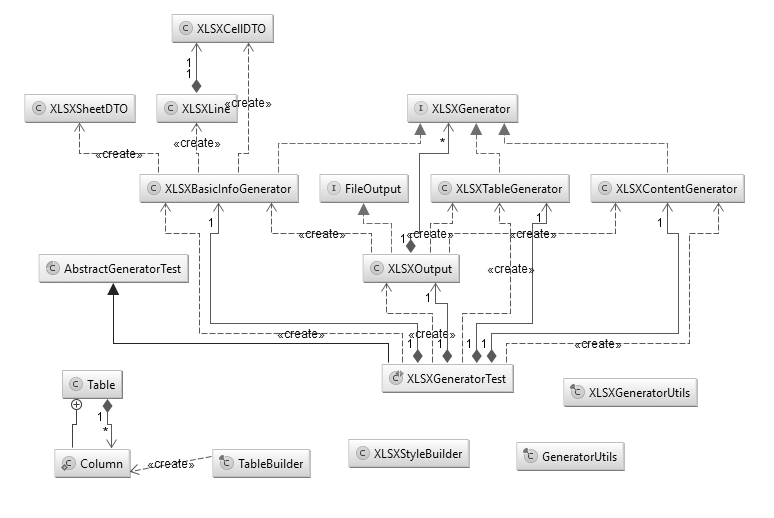
\includegraphics[scale=0.8]{core_output}
	\centering
	\caption{Schéma generátoru XLSX \label{fig:core_output}}
\end{figure} 
\FloatBarrier

Tento balíček obsahuje, jako jediný, jednotkové testy. Je zde vytvořen mock proběhnuté analýzy a podle něj jsou generovány soubory. Testy ale nejsou spouštěny při sestavování programu, spíše jsou zde pro ulehčení a zrychlení vývoje.


\section{Modul Fxml}
Modul FXML je pomocný modul pro práci s JavaFX, který pak dále využívá modul Application a Dev. Obsahuje pouze několik společných třídy pro tyto dva moduly, schéma je vidět na obrázku \ref{fig:fxml_whole}. JavaFX vytváří \gls{glos:GUI} pomocí speciálního XML formátu FXML nebo je možné využít i programátorský přístup a udělat vše manuálně. Pro vytvoření nového prvku je potřeba znát název FXML souboru a také jeho kontrolor, aby se nemuselo pokaždé tyto dvě věci definovat, tak třída FXApplication obsahuje metody pro tvorbu nových prvků a přepínání kontextu. Stáčí tedy definovat nový prvek v enumu FXMLElement a zavolat patřičnou metodu v FXApplication. Ta vezme prvek z enumu a pomocí FXMLCreator vytvoří nový prvek, k němuž je pak přiřazen abstraktní kontrolor. Jediná podmínka je pak ta, že každý kontrolor musí být potomkem abstraktního předka a v aplikaci pak proběhne přetypování na konkrétní kontrolor.

\begin{figure}[h]
	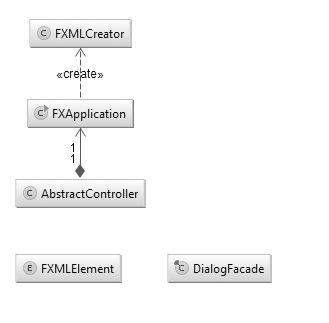
\includegraphics[scale=0.9]{fxml_whole}
	\centering
	\caption{Schéma modulu FXML \label{fig:fxml_whole}}
\end{figure} 
\FloatBarrier

Při vytváření elementu ve třídě FXMLCreator se také nastavuje cesta k lokalizačním souborům, ta se bere z MessageUtils, který je v modulu Core. Aplikace je tímto uzpůsobena na možnost více jazyků. V této třídě je možné vytvořit i element, který bude spolupracovat s \gls{glos:CDI}. Toho bylo využito téměř po celou dobu vývoje aplikace a byla zvolena implementace WeldSE. Ale po problémech s pomalejším načítáním programu a pro zvláštní chování s použitím ProGuard a Shade pluginu pro Maven bylo od této implementace opuštěno (funkce těchto pluginů je popsána v kapitole \ref{sec:app}). Tímto bohužel aplikace ztratila interceptory pro kontrolování výkonu jednotlivých metod, snazší logování programu pomocí log4j, řešení automatických závislostí a lepší práci se singletone objekty. Do dalšího možného vývoje práce je možné zkusit CDI implementovat pomocí Spring Boot, který by neměl dělat problémy, které vznikaly při použití WeldSE. A to zejména proto, že není definován pomocí XML, ale konfigurace se provádí přímo v Jave.

\section{Modul Application}\label{sec:app}
V modulu Application je definováno uživatelské rozhraní a komunikace s modulem Core. Aplikace je založena na návrhovém vzoru \gls{glos:MVC}. Jedná se pouze o několik kontrolorů a pomocných tříd, bez žádné složitější logiky, tu pak obstarává modul Core. Hlavním kontrolorem je třída MainController, jehož rozhraní je vidět na obrázku \ref{fig:app_main}. Práce s programem je zobrazena na obrázku \ref{fig:flow}.

\begin{figure}[h]
	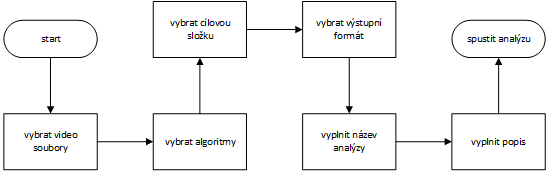
\includegraphics[scale=0.9]{flow}
	\centering
	\caption{Průběh práce s programem \label{fig:flow}}
\end{figure} 
\FloatBarrier

\begin{figure}[h]
	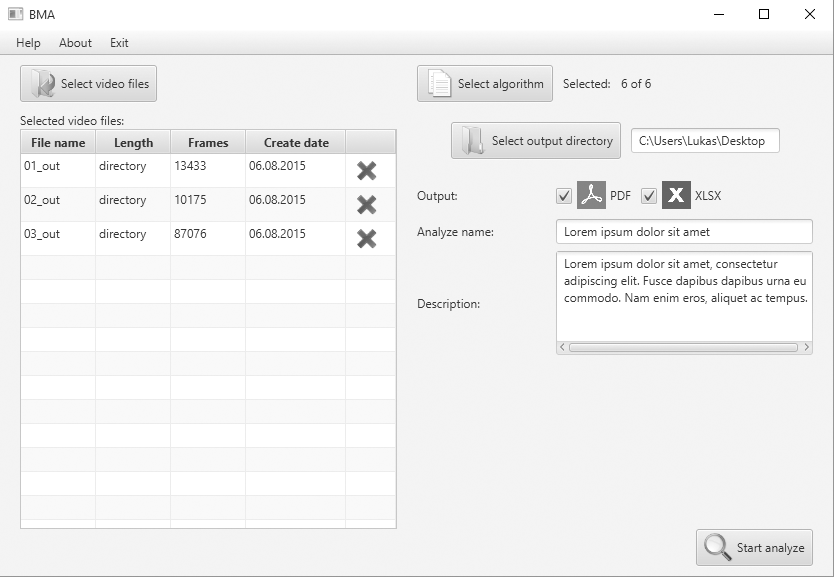
\includegraphics[scale=0.7]{app_main}
	\centering
	\caption{Hlavní obrazovka aplikace \label{fig:app_main}}
\end{figure} 
\FloatBarrier


Z hlavní obrazovky se dá spustit AlgorithmManagerController, viz. obrázek \ref{fig:app_manager}. Kde se vyberou konkrétní algoritmy, které se mají použít pro aktuální analýzu. Dále se na hlavní obrazovce dá zvolit, které soubory se budou zpracovávat a kam se pak vygenerují výstupní soubory. Lze k analýze připsat i volitelné doplňkové údaje, ty se pak také vygenerují k výstupním souborům. Po spuštění analýzy je zobrazen dialog průběhu, který je vidět na obrázku \ref{fig:app_progress}.

\begin{figure}[h]
	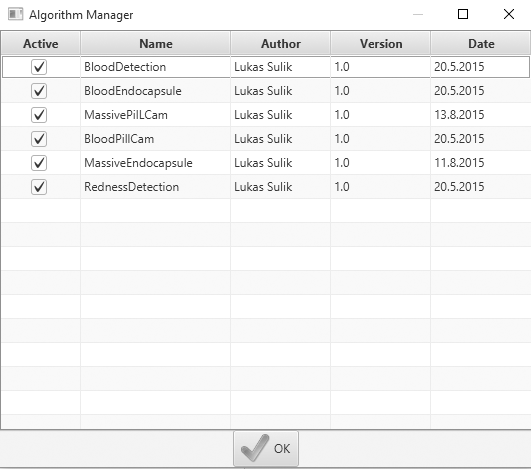
\includegraphics[scale=0.9]{app_manager}
	\centering
	\caption{Správa algoritmů \label{fig:app_manager}}
\end{figure} 
\FloatBarrier

ProgressDialogController implementuje rozhraní ProgressNotifier z modulu Core. Přes toto rozhraní jsou posílány signály z asynchronního zpracování souborů a na základě toho je v tomto případě aktualizováno uživatelské rozhraní. Při implementování jiného \gls{glos:GUI} je možné využít toto rozhraní jinak, např. pokud by se jednalo o webovou aplikaci, tak je možné ukládat záznam o průběhu do databáze a uživatel by se pak na něj mohl dotazovat pomocí ajaxových dotazů.

\begin{figure}[h]
	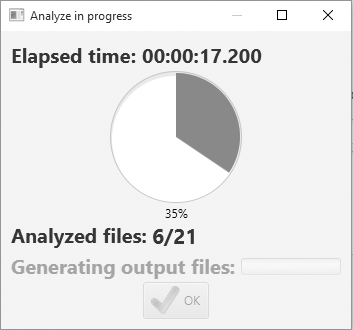
\includegraphics[scale=0.9]{app_progress}
	\centering
	\caption{Dialog průběhu \label{fig:app_progress}}
\end{figure} 
\FloatBarrier

V modulu application jsou umístěné Maven skripty pro sestavování programu. Nejprve je využit Maven Shade plugin, který dle definice autoru - "Tento plugin má schopnost zabalit program do uber-jar, včetně jeho závislostí a zastínit ho - tj. přejmenovat balíčky nějakých závislostí." volně přeloženo z \cite{apache}. Plugin také odstraňuje duplicitní závislosti, to může vznikat v případě, že různé knihovny využívají další knihovny, které mohou být stejné. Dále je spuštěn ProGuard plugin, ten má definovanou konfiguraci v externím souboru a v Mavenu se pouze spustí. Z tohoto pluginu je využita pouze obfuskace kódu, ostatní možnosti jsou zakázány. Až na pár vyjímek nutných k funkčnosti je obfuskován celý kód a s ním i knihovna OpenCV, ukázka výsledku je na obrázku \ref{fig:app_obfus}.

\begin{figure}[h]
	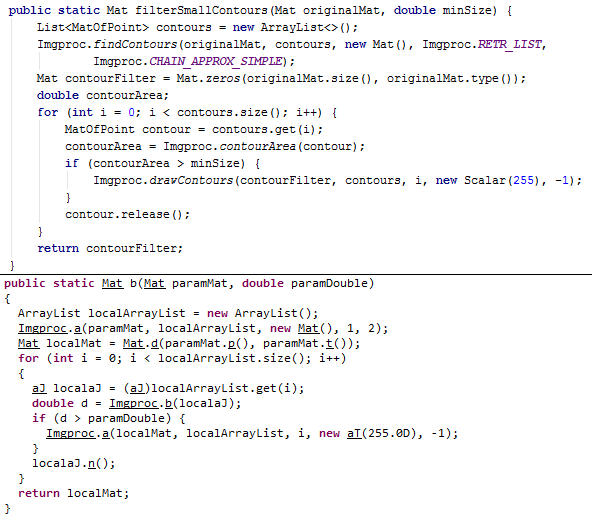
\includegraphics[scale=0.9]{app_obfus}
	\centering
	\caption{Horní část ukázky je zdrojový kód. Dolní je dekompilovaný obfuskovaný kód. \label{fig:app_obfus}}
\end{figure} 
\FloatBarrier

Jakmile je připravena JAR knihovna, spustí se plugin Launch4J, který vytvoří spouštěcí soubor pro platformu Windows. Je možné spouštět aplikaci i přes JAR, jelikož je odděleno od exe souboru, ale takto je to pohodlnější pro uživatele Windows. V exe souboru je také zakomponována kontrola minimální verze Javy.

\section{Modul Dev}
Modul Dev slouží pouze k vývoji algoritmů a není zahrnut do sestavení aplikace pro uživatele. Vznikl proto, že autor nemohl nalézt žádné vývojové nástroje pro Javu, které by byly kompatibilní s OpenCV a byly vhodné pro účel práce. Obsahuje pouze prosté \gls{glos:GUI}, které se z větší části generuje pomocí reflexe. Aby bylo možné pracovat s algoritmy v reálném čase a sledovat tak přímo, co který algoritmus s určitou konfigurací na konkrétním snímku dělá bylo nutné zasáhnout do logiky programu. Je snaha tento zásah řešit pouze v tomto modulu, ale některé nutné úpravy byly udělány i ve třídě Buffer (neomezená kapacita a nemažou se data) a VideoFrame(metody pro ukládání snímku algoritmu), fungují však pouze pokud je globálně zapnutý vývojový mód, a tak není ovlivněn běžný chod programu.

V rozhraní je stejně tak jako v aplikaci spuštěn MainController, který obsahuje jen volbu algoritmu a souboru, který má být zpracován, lze zpracovávat pouze jeden soubor a algoritmus najednou. Po spuštění programu je vystavěno vývojové rozhraní, které je vidět na obrázku \ref{fig:dev_debug}. Pomocí reflexe jsou získána všechna pole z třídy a ta, která obsahují anotaci @DevInterfaceField (ukázka na obrázku \ref{fig:core_new}), se zpracují a vytvoří se z nich ovládací prvek na základě hodnoty v atributu fieldType. Ovládací prvky mohou být: zaškrtávací políčko (pro booelan), posuvník (int, double, ...), obyčejné pole (string, int, ...) a výčtový typ. Výčtový typ je použit pro ukládání snímku algoritmu v daném kroku např. obrázek \ref{fig:dev_enum}.

\begin{figure}[h]
	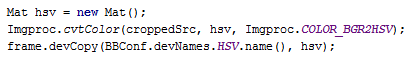
\includegraphics[scale=0.9]{dev_enum}
	\centering
	\caption{Ukázka konverze z BGR do HSV a následné uložení snímku pro vývoj. \label{fig:dev_enum}}
\end{figure} 
\FloatBarrier

\begin{figure}[h]
	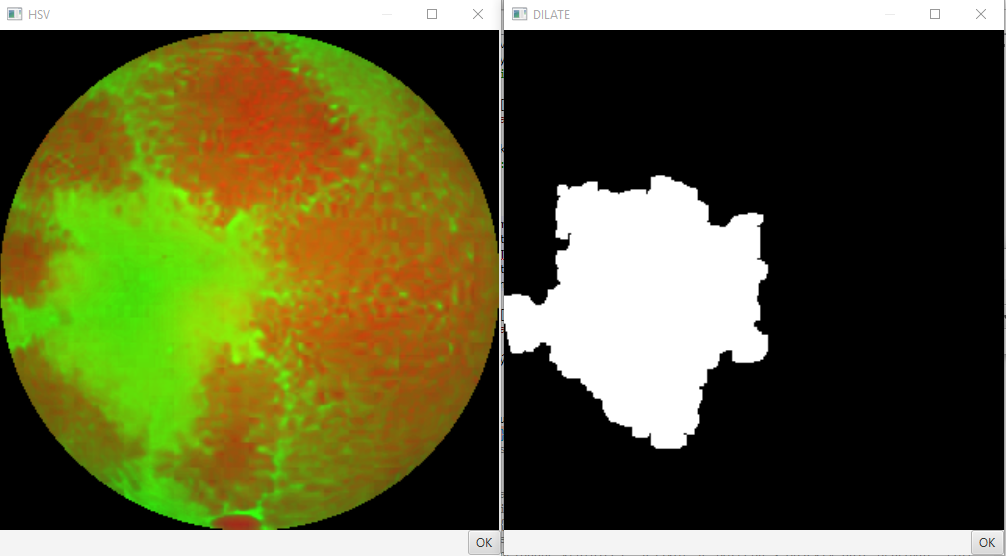
\includegraphics[scale=0.4]{dev_snap}
	\centering
	\caption{Ukázka snímků algoritmu. Vlevo převod do HSV, vpravo dilatace. \label{fig:dev_snap}}
\end{figure} 
\FloatBarrier

Pro běh programu je spuštěn AnalyzeTask z modulu Core pro získání a zpracování dat. K tomu je spuštěno další vlákno, kde běží BufferPlayer, který je potomkem AbstractBufferTask z modulu Core. Ten zpracovává data z Bufferu s aktuální konfigurací a také zobrazuje vybraná data snímků algoritmu v rozhraní, na obrázku \ref{fig:dev_snap} jsou vidět snímky z algoritmu. BufferPlayer také ukládá všechny detekované artefakty a k nim i snímky na disk pro rychlejší orientaci, co je detekováno. Jak je vidět na obrázku \ref{fig:dev_debug}, tak rozhraní disponuje ještě pauzou, posuvníkem rychlosti, opakováním a přechodem na konkrétní snímek v bufferu.



\begin{figure}[h]
	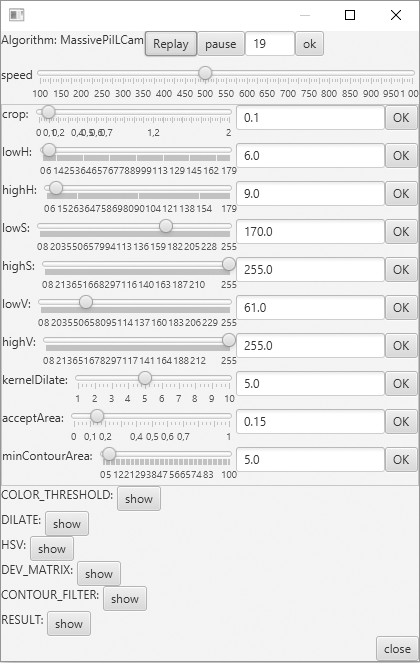
\includegraphics[scale=0.9]{dev_debug}
	\centering
	\caption{Vývojové rozhraní konkrétního algoritmu. \label{fig:dev_debug}}
\end{figure} 
\FloatBarrier

